\documentclass[t,12pt]{beamer}
\definecolor{links}{RGB}{0, 104, 172}
\definecolor{red}{rgb}{0.702,0.106,0.106} 
\hypersetup{colorlinks=true,urlcolor=links}
\usetheme{default}
% we need to change to Cornell red
\definecolor{beamer@blendedblue}{rgb}{0.702,0.106,0.106} 
\beamertemplatenavigationsymbolsempty
\setbeamerfont{institute}{size={\fontsize{10}{10}}}

\usepackage[english]{babel}
\usepackage{textgreek}
\usepackage{fontspec}
\setsansfont{TeX Gyre Heros}

\title{HD4630 Workshop I}
\subtitle{Preprocessing \& First-Level Analysis}
\author{Elizabeth DuPre \\[.8\baselineskip]}

\vspace{2ex}
\institute{Human Neuroscience Institute 
\\[4pt]
\href{http://www.human.cornell.edu/hd/}{Department of Human Development}
\\[4pt]
\href{https://www.cornell.edu/}{Cornell University}}
\date{}

\begin{document}
% Title Slide
\begin{frame}
  \titlepage
\end{frame}

\section{Introduction}
% First Slide
\begin{frame}{Why Preprocess?}
\vspace{10pt}
\begin{itemize}
\setlength\itemsep{1em}
  \item fMRI data is acquired with physical, biological constraints
  \vspace{4pt}
  \begin{itemize}
  \setlength\itemsep{0.5em}
   \item MRI machines aren't magic!
   \item Sampling neural activity in living, breathing \\ human beings
  \end{itemize}
  \item We need to compare data across participants \\ to draw (statistically) meaningful conclusions
\end{itemize}
\end{frame}

% Second Slide
\begin{frame}{Basic Preprocessing}
\vspace{10pt}
\begin{itemize}
\setlength\itemsep{1em}
\item Discard pre-steady state TRs
\item Slice-timing correction
\item Rigid-body motion correction
\item Coregistration of functional \& anatomical
\item Normalization to standard template
\item Spatial filtering (Smoothing)
\end{itemize}
\end{frame}

% Third Slide
\begin{frame}{Preprocessing in AFNI}
\vspace{10pt}
\begin{itemize}
\setlength\itemsep{1em}
\item AFNI allows you to see as little (or as much) detail \\ as you want when preprocessing
\item In this class, we'll be using \texttt{uber\textunderscore{}subject.py}, a preprocessing GUI that hides many technical \\ details
\vspace{4pt}
\begin{itemize}
\item To see what's happening, we'll have to look at the generated \texttt{tcsh} script
\end{itemize}
\end{itemize}
\end{frame}

% Fourth Slide
\begin{frame}{First-level Analysis}
\vspace{10pt}
\begin{itemize}
\setlength\itemsep{1em}
\item \texttt{uber\textunderscore{}subject.py} also includes first-level analysis
\item First-level analysis involves estimating the \textbeta{}-matrix in
\begin{eqnarray*}
Y = X\beta + \epsilon
\end{eqnarray*}
by constructing the contrast matrix X
\item A great review of the math underlying this is available from \href{http://mumfordbrainstats.tumblr.com/post/125163337126/day-4-multiple-linear-regression}{Mumford Brain Stats}
\end{itemize}
\end{frame}

% Fifth Slide
\begin{frame}{Plan for Today}
\vspace{10pt}
\begin{itemize}
\setlength\itemsep{1em}
\item Review, with examples, basic preprocessing
\item Discuss first-level analysis in a traditional general linear model (GLM) framework
\item Work along in AFNI using \texttt{uber\textunderscore{}subject.py}
\vspace{4pt}
\begin{itemize}
\setlength\itemsep{0.5em}
\item Preprocess a participant from OpenfMRI \\ ds000102 (Flanker task)
\item Perform a first-level analysis for incongruent vs. congruent Flanker trials
\end{itemize}
\end{itemize}
\end{frame}

% Sixth Slide
\begin{frame}{Launching the Docker Container}
\vspace{10pt}
\begin{itemize}
\setlength\itemsep{1em}
\item We want you to run this locally, so you'll need to launch the docker image you downloaded
\item The full instructions to do so are on the \href{https://emdupre.github.io/hd4630_workshops/categories}{course website}, but as a quick reminder:
\vspace{4pt}
\begin{itemize}
\setlength\itemsep{0.5em}
\item For Mac: execute \texttt{mac\textunderscore{}launch.sh} in a terminal with Docker running
\item For Windows: execute \texttt{windows\textunderscore{}ip.cmd} in a command prompt. Then, supply that IP to \texttt{windows\textunderscore{}launch.sh} in a Docker Quickstart Terminal
\end{itemize}
\end{itemize}
\end{frame}

\section{Preprocessing}
% Seventh Slide
\begin{frame}{First Steps: Looking at the Data}
\vspace{10pt}
\begin{itemize}
\setlength\itemsep{1em}
\item No matter what you're doing, this is the first step! 
\item Here, we'll need to look at both our anatomical and functional images
\end{itemize}
\vspace{4pt}
\centering
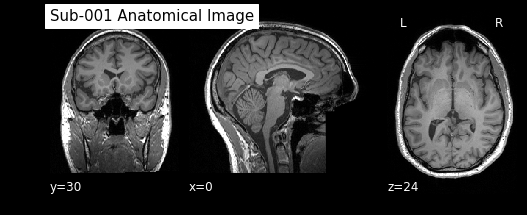
\includegraphics[width=.6\textwidth]{images/sub-001_anat_image.png} \\
\vspace{4pt}
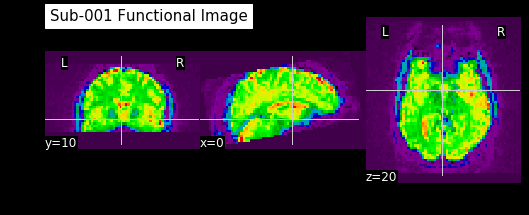
\includegraphics[width=.6\textwidth]{images/sub-001_func_image.png} \\
\end{frame}

% Eighth Slide
\begin{frame}{\emph{To Do}: Open Data in AFNI}
\vspace{10pt}
\begin{itemize}
\setlength\itemsep{1em}
\item Type \texttt{afni} into the terminal window to open a new session
\item For sub-01 of the Flanker task:
\vspace{4pt}
\begin{itemize}
\setlength\itemsep{0.5em}
\item Read in the \texttt{anat} directory
\item Read in the \texttt{func} directory and \\ scroll through the time series of one run
\item Close \texttt{afni}
\end{itemize}
\end{itemize}
\end{frame}

% Ninth Slide
\begin{frame}{What Happened to My Anatomical Image?}
\vspace{10pt}
\begin{itemize}
\setlength\itemsep{1em}
\item Defacing is a common step in publicly available MRI data
\item Intended to reduce the risk of participant identification
\end{itemize}
\vspace{4pt}
\centering
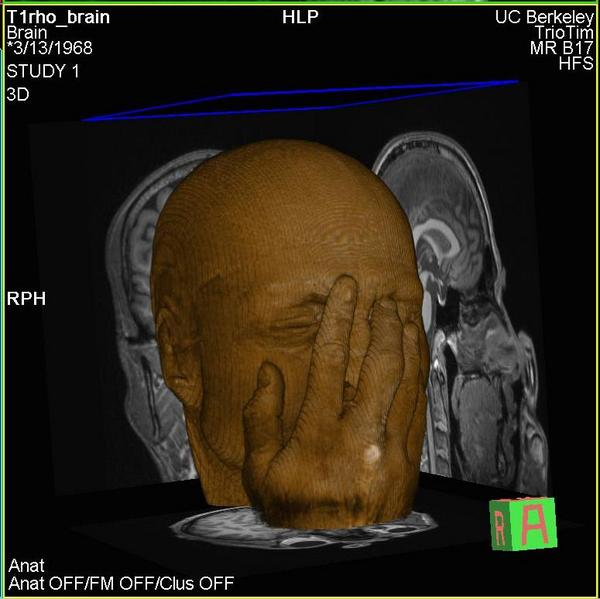
\includegraphics[width=.5\textwidth]{images/practiCalfMRI_facepalm.jpg}
\end{frame}

% Tenth Slide
\begin{frame}{Discard Pre-Steady State TRs}
\vspace{10pt}
\begin{itemize}
\setlength\itemsep{1em}
\item Pre-steady state or unsaturated volumes show vastly different properties from the rest of an EPI series
\item Because of this, some scanners do not reconstruct these "dummy scans" by default
\vspace{4pt}
\begin{itemize}
\setlength\itemsep{0.5em}
\item Both of our OpenfMRI datasets exclude pre-steady state volumes, so we will not discard any TRs
\end{itemize}
\end{itemize}
\end{frame}

% Eleventh Slide
\begin{frame}{\emph{To Do}: Open \texttt{uber\textunderscore{}subject.py}}
\centering
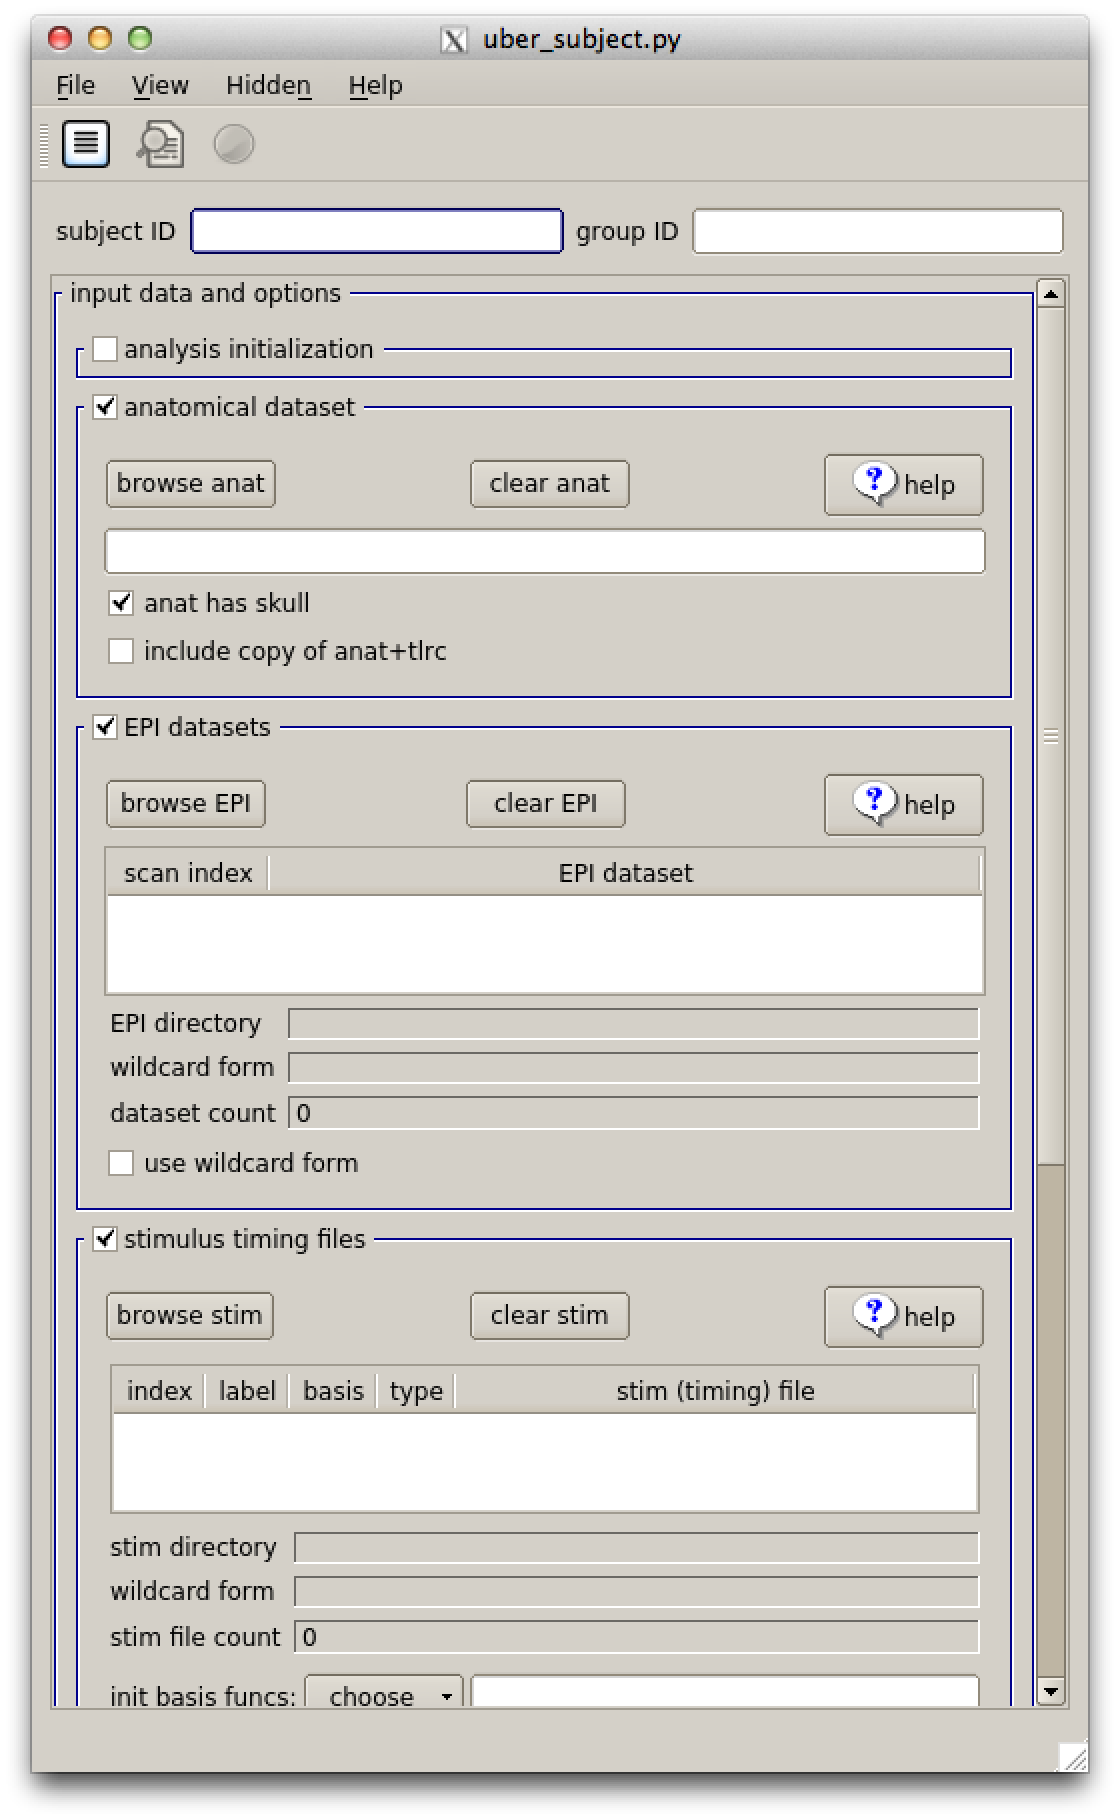
\includegraphics[width=.65\textwidth]{images/uber_subject.png}
\end{frame}

% Twelfth Slide
\begin{frame}{Slice Timing Correction}
\vspace{10pt}
\begin{itemize}
\setlength\itemsep{1em}
\item In single-shot EPI, each slice in a volume is acquired at a different time
\item In our Flanker task, slices were acquired over a 2000ms TR in an interleaved fashion
\end{itemize}
\centering{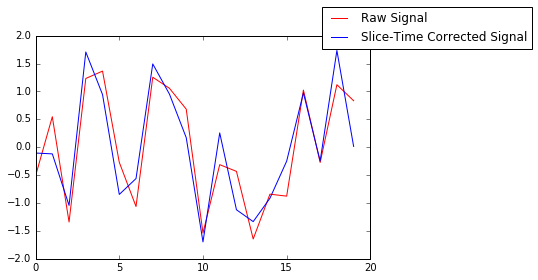
\includegraphics[width=.7\textwidth]{images/slice_timing_corr.png}}
\end{frame}

% Thirteenth Slide
\begin{frame}{\emph{To Do}: Slice Timing}
\vspace{10pt}
\begin{itemize}
\setlength\itemsep{1em}
\item By default, AFNI will check the image header for slice timing information
\item You can change the default interpolation used, but we won't address that in this workshop 
\end{itemize}
\end{frame}

% Fourteenth Slide
\begin{frame}{Rigid-Body Motion Correction}
\vspace{10pt}
\begin{itemize}
\setlength\itemsep{1em}
\item AFNI will estimate and correct for movement across the entire scan
\end{itemize}
\vspace{4pt}
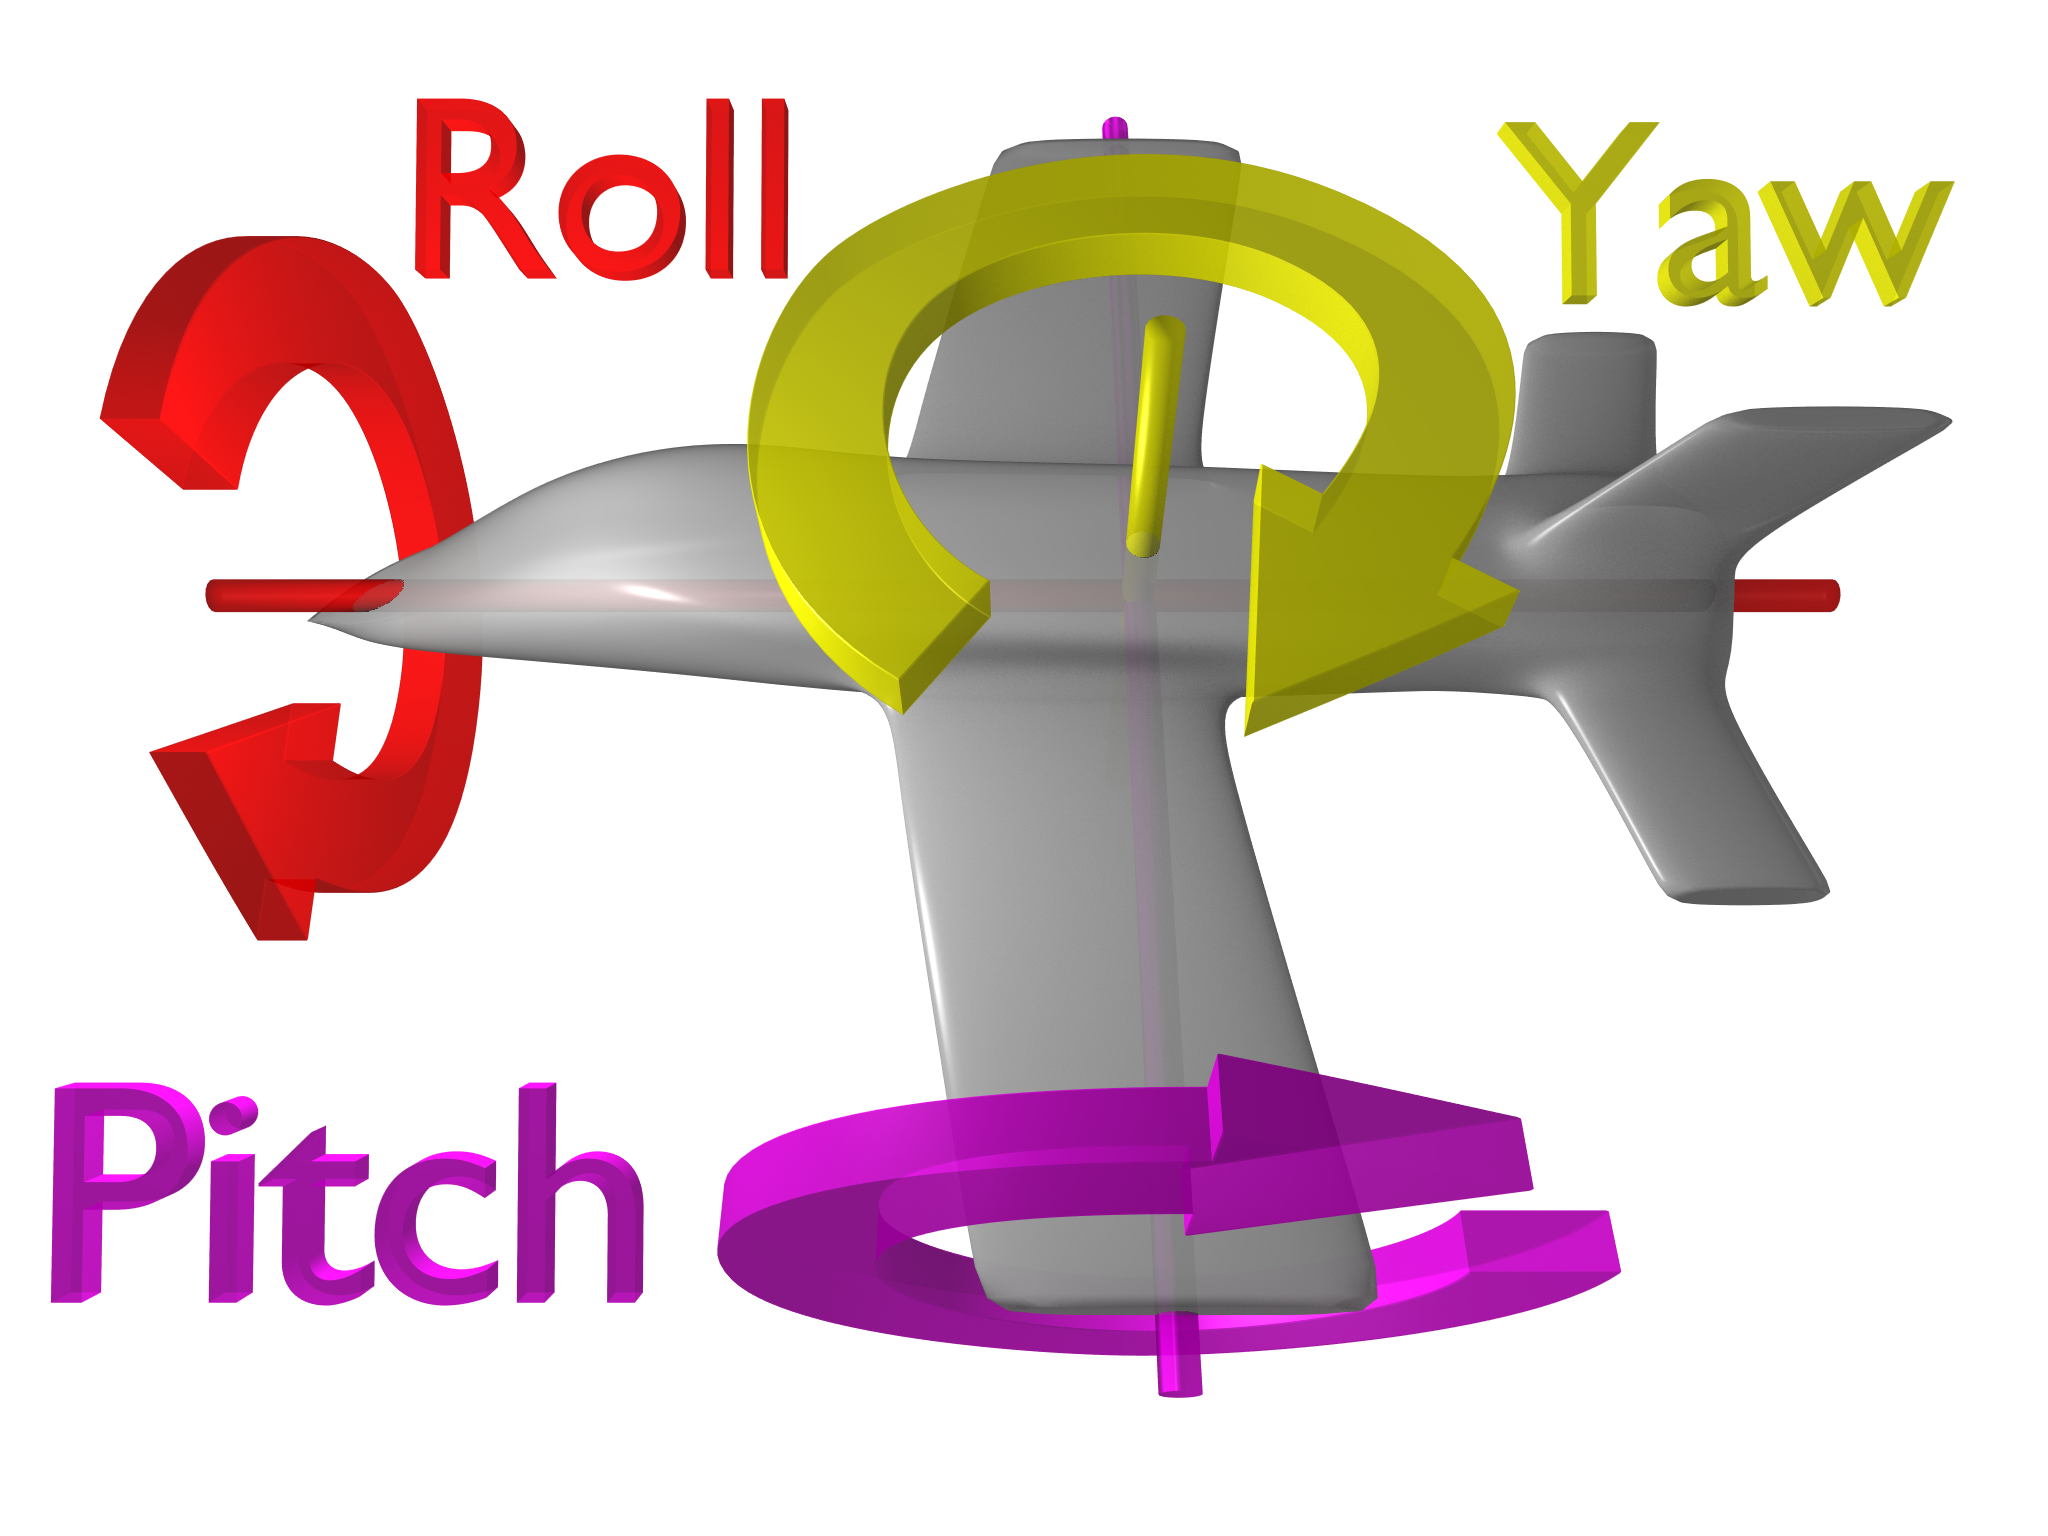
\includegraphics[width=.5\textwidth]{images/Flight_dynamics_with_text.png}
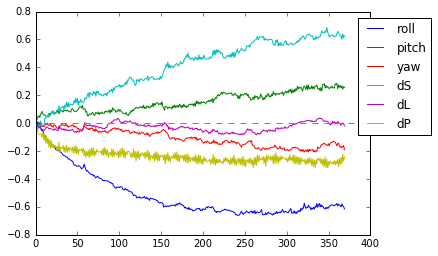
\includegraphics[width=.5\textwidth]{images/motion_regressors.png}
\centering
\vspace{10pt}
\textit{This is a well-behaved participant!}
\end{frame}

% Fifteenth Slide
\begin{frame}{\emph{To Do}: Set Volume Registration Base}
\vspace{10pt}
\begin{itemize}
\setlength\itemsep{1em}
\item To perform rigid body motion correction, we need \\ to select a volume to which to register all other volumes
\item Since we did not remove any pre-steady state TRs, we can set this option to 'first'
\end{itemize}
\end{frame}

% Sixteenth Slide
\begin{frame}{The Limits of Motion Correction}
\vspace{10pt}
\begin{itemize}
\setlength\itemsep{1em}
\item Movement is a \emph{major} concern in fMRI analysis
\item Participants who show high levels of movement \\ may not be usable
\vspace{4pt}
\begin{itemize}
\item Even when correcting for motion, subtle differences may remain
\end{itemize}
\end{itemize}
\end{frame}

% Seventeenth Slide
\begin{frame}{}
\vspace{10pt}
\centering
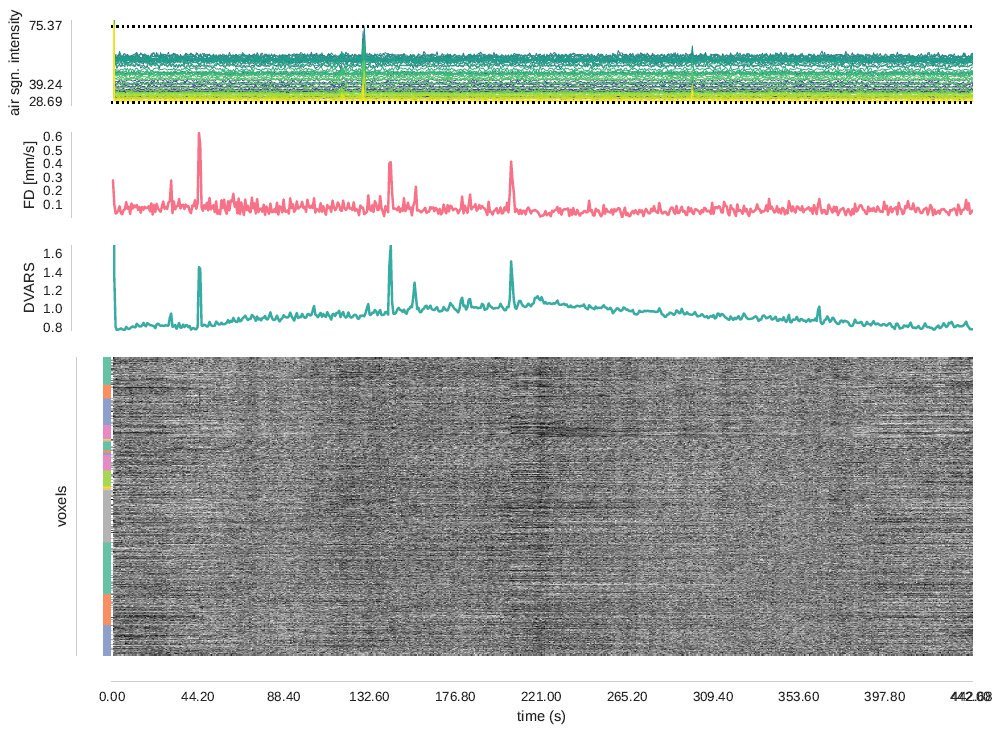
\includegraphics[width=\textwidth]{images/mriqc_plot.jpg} \\
\vspace{-10pt}
\begin{block}{}
Visualization from \href{http://mriqc.readthedocs.io/en/latest/index.html}{MRIQC}
\end{block}
\end{frame}

% Eighteenth Slide
\begin{frame}{\emph{To Do}: Set Motion Censoring}
\vspace{10pt}
\begin{itemize}
\setlength\itemsep{1em}
\item 'Motion censor limit' sets the maximum amount of motion allowed in any one TR
\item TRs showing motion higher than this limit are 'scrubbed' from the time series
\end{itemize}
\end{frame}

% Nineteenth Slide
\begin{frame}{Coregistration}
\vspace{10pt}
\begin{itemize}
\setlength\itemsep{1em}
\item We need to get the functional and anatomical images into the same space
\item By default, these are likely to be out of alignment as participants move between scans
\vspace{4pt}
\begin{itemize}
\setlength\itemsep{0.5em}
\item After motion correction, all of our functional images should be aligned to one another
\item Aligning these to the anatomical image should therefore be a one step correction
\end{itemize}
\end{itemize}
\end{frame}

% Twentieth Slide
\begin{frame}{}
\vspace{10pt}
\centering
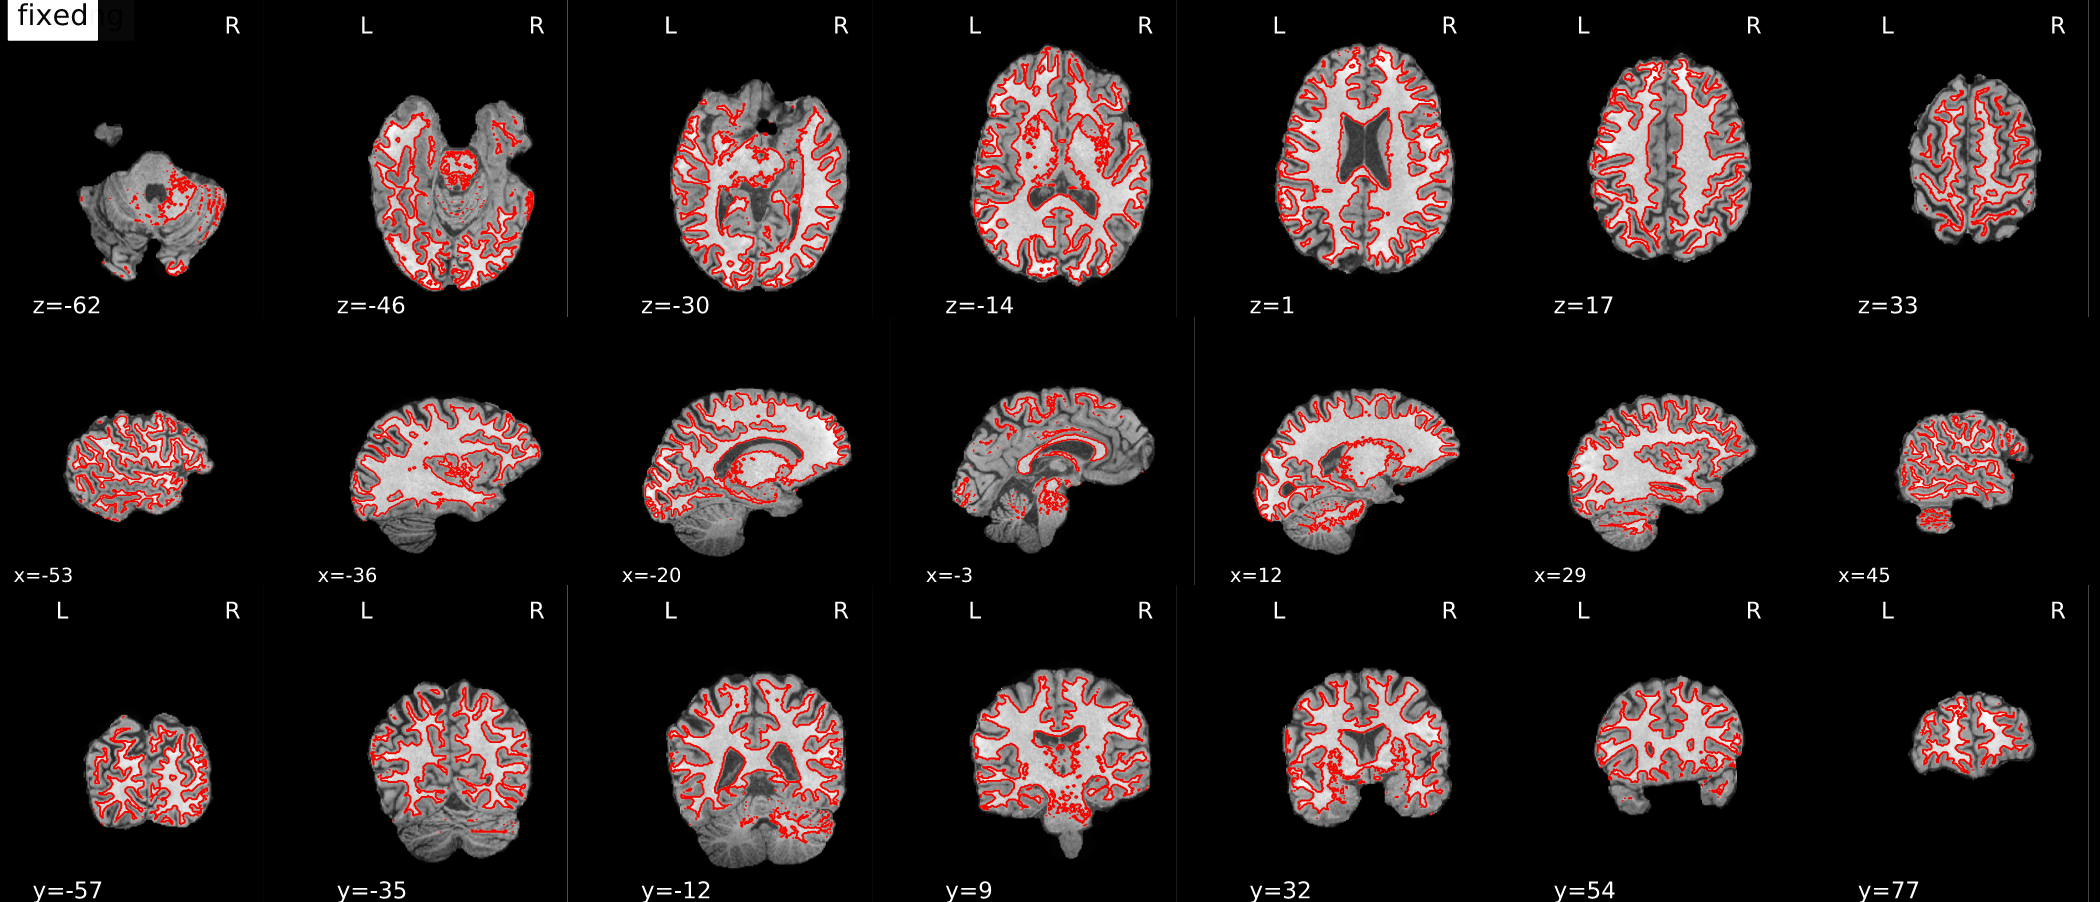
\includegraphics[width=.85\textwidth]{images/fixed_coreg.png} \\
\vspace{4pt}
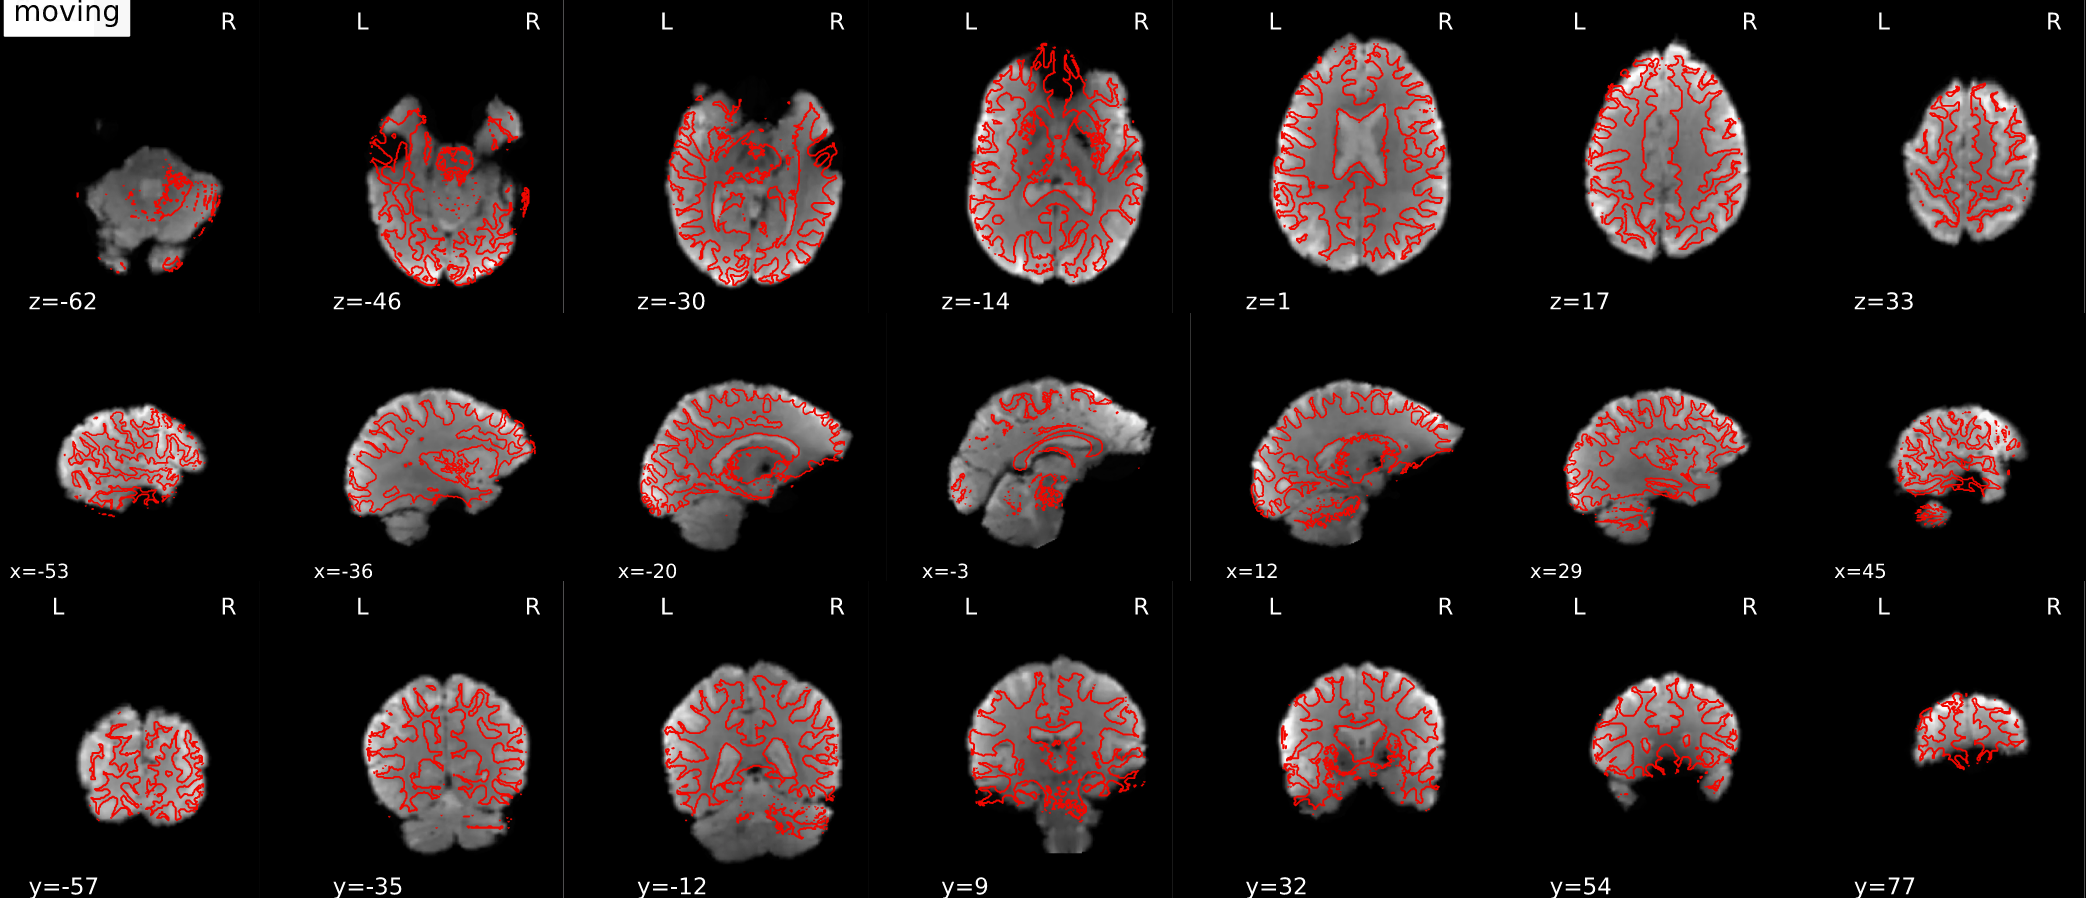
\includegraphics[width=.85\textwidth]{images/moving_coreg.png} \\
\vspace{-10pt}
\begin{block}{}
Visualization from \href{http://fmriprep.readthedocs.io/en/stable/}{fMRIPrep}
\end{block}
\end{frame}

% Twenty-first Slide
\begin{frame}{\emph{To Do}: Extra Alignment Options}
\vspace{10pt}
\begin{itemize}
\setlength\itemsep{1em}
\item 'Local Pearson Correlation' is the default coregistration option
\vspace{4pt}
\begin{itemize}
\item This is appropriate for T1 to EPI registration, but may need to be changed for other modalities
\end{itemize}
\item Select 'use giant\textunderscore{}move' to allow AFNI to align anatomical and functional images where participants have moved substantially
\end{itemize}
\end{frame}

% Twenty-second Slide
\begin{frame}{Normalization}
\vspace{10pt}
\begin{minipage}{.49\textwidth}
\begin{itemize}
\setlength\itemsep{1em}
\item Standard templates currently in use include Talaraich and MNI
\vspace{4pt}
\begin{itemize}
\setlength\itemsep{0.5em}
\item MNI based on many living subjects \\ rather than one post-mortem
\item Several different versions of the MNI are in use!
\end{itemize}
\end{itemize}
\end{minipage}
\begin{minipage}{.49\textwidth}

\includegraphics[width=\textwidth]{images/king_bob.png} \\
\end{minipage}
\end{frame}

% Twenty-third Slide
\begin{frame}{\emph{To Do}: Extra TLRC Options}
\vspace{10pt}
\begin{itemize}
\setlength\itemsep{1em}
\item 'TLRC' is short for Talaraich, the default normalization space in AFNI
\item Change this to \texttt{MNI\textunderscore{}avg152T1} to align our subject to MNI space
\vspace{4pt}
\begin{itemize}
\item This corresponds to the MNI 2009c nonlinear template
\end{itemize}
\end{itemize}
\end{frame}

% Twenty-fourth Slide
\begin{frame}{Spatial Filtering (Smoothing)}
\vspace{10pt}
\begin{enumerate}
\setlength\itemsep{1em}
\item Increases signal-to-noise ratio
\item Helps to ameliorate residual anatomical variability
\item Allows data to meet assumptions of Gaussian Random Field theory
\vspace{4pt}
\begin{itemize}
\item A fun introduction to this is provided in \href{http://www.fil.ion.ucl.ac.uk/~wpenny/mbi/chance3.pdf}{Worsley, 1996}
\end{itemize}
\end{enumerate}
\vspace{4pt}
\centering
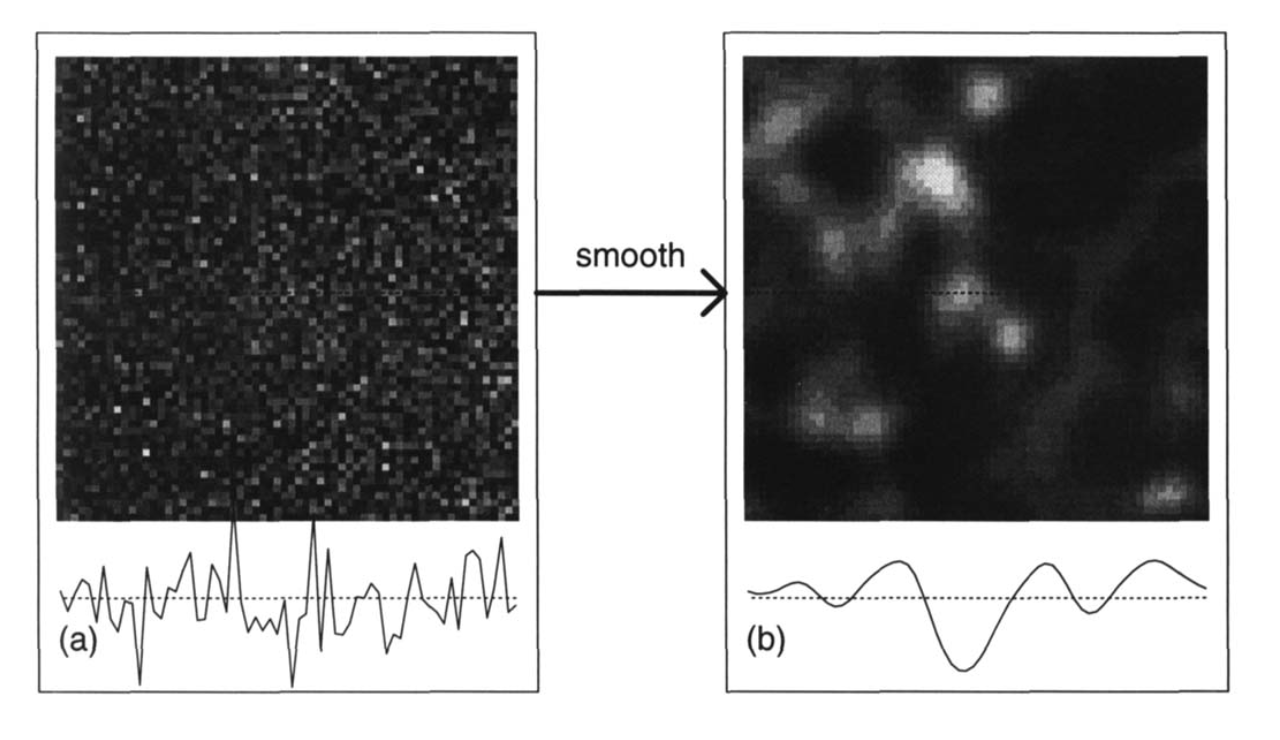
\includegraphics[width=.65\textwidth]{images/gaussian_smoothing.png} \\
\end{frame}

% Twenty-fifth Slide
\begin{frame}{\emph{To Do}: Set Blur Size}
\vspace{10pt}
\begin{itemize}
\setlength\itemsep{1em}
\item We need to specify the FWHM (Full-Width at Half-Maximum) of our Gaussian kernel
\item 4mm is the default, but we'll increase this to 6mm (FWHM $\geq$ 2x voxel size)
\end{itemize}
\end{frame}

% Twenty-sixth Slide
\begin{frame}{Inspecting our Script}
\vspace{10pt}
\begin{itemize}
\setlength\itemsep{1em}
\item Now that we have preprocessing set up, we can look at the parameters for our example subject
\end{itemize}
\vspace{4pt}
\begin{minipage}[t]{0.39\textwidth}
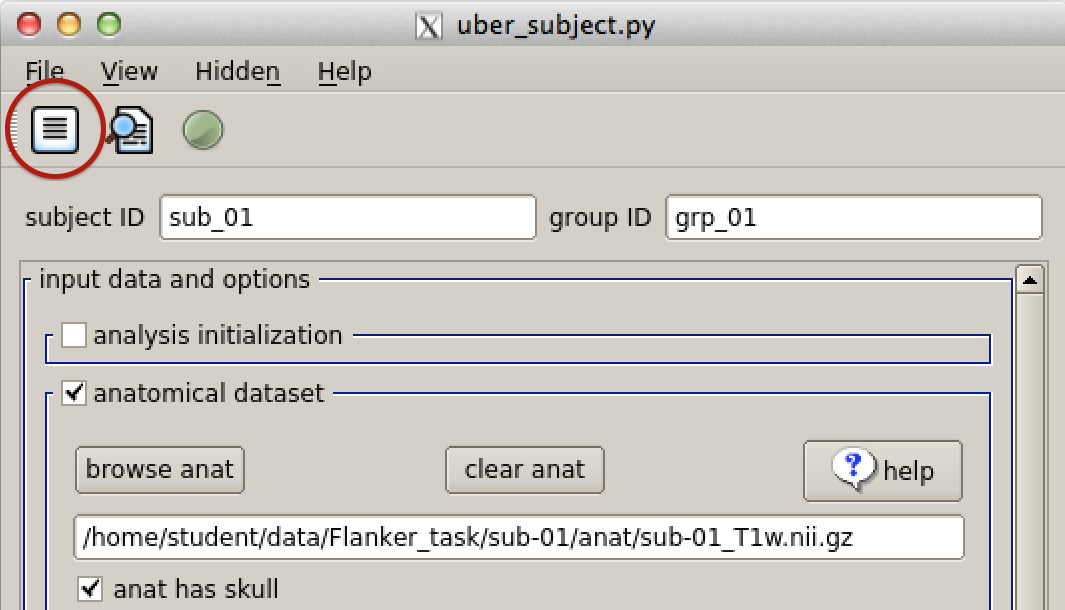
\includegraphics[width=\textwidth]{images/gen_afni_proc.png} \\
\end{minipage}
\begin{minipage}{0.59\textwidth}
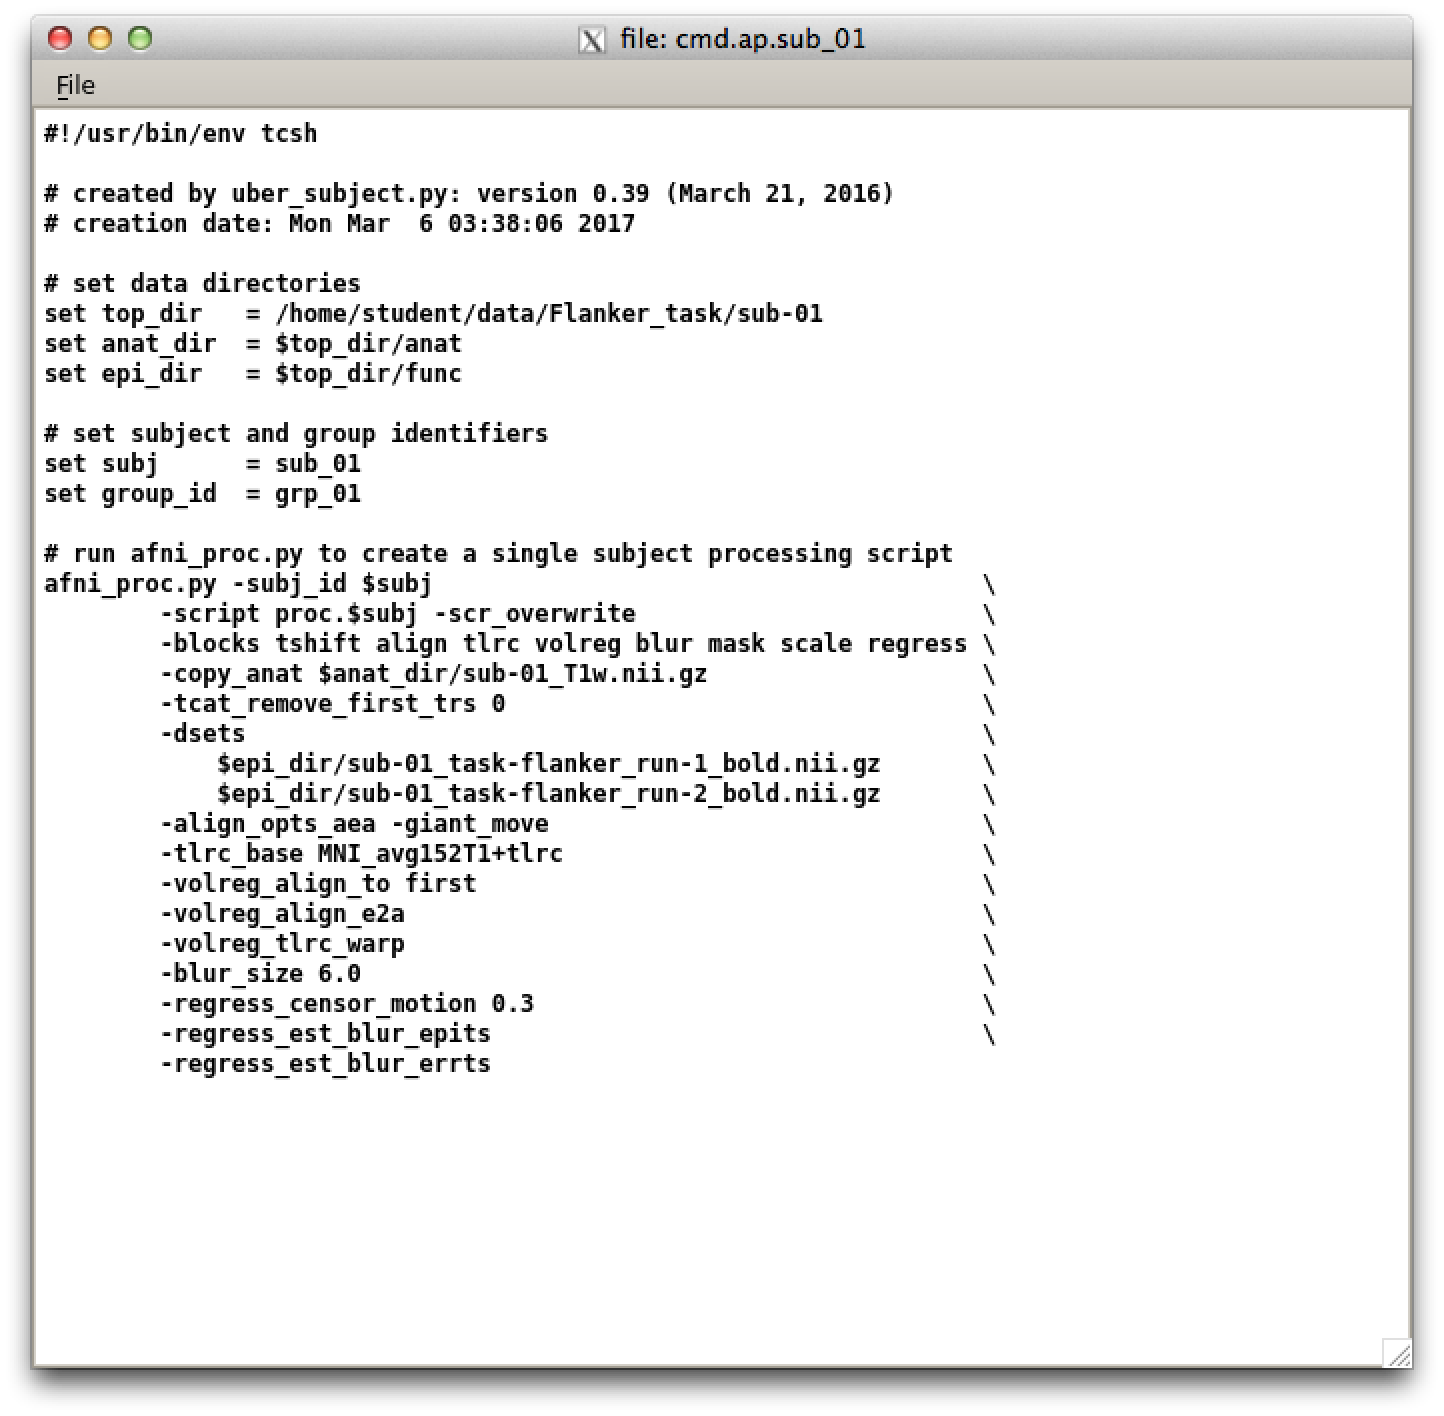
\includegraphics[width=\textwidth]{images/afni_proc.png} \\
\end{minipage}
\end{frame}

% Twenty-seventh Slide
\section{First-level Analysis}
\begin{frame}{First-Level Analysis}
\vspace{10pt}
\begin{itemize}
\setlength\itemsep{1em}
\item \texttt{uber\textunderscore{}subject.py} also incorporates first-level analysis
\item For this, we'll need to know the stimulus timing for each of the conditions in the Flanker task
\vspace{4pt}
\begin{itemize}
\item We'll collapse the two 'congruent' and 'incongruent' conditions, ignoring participant accuracy
\end{itemize}
\end{itemize}
\vspace{4pt}
\centering
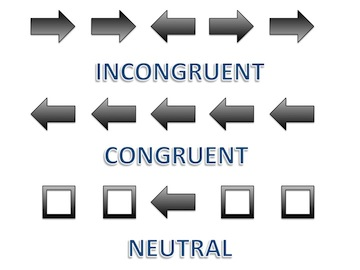
\includegraphics[width=.5\textwidth]{images/flanker_task.jpg}
\end{frame}
\end{document}


